%% 
%% Copyright 2007-2025 Elsevier Ltd
%% 
%% This file is part of the 'Elsarticle Bundle'.
%% ---------------------------------------------
%% 
%% It may be distributed under the conditions of the LaTeX Project Public
%% License, either version 1.3 of this license or (at your option) any
%% later version.  The latest version of this license is in
%%    http://www.latex-project.org/lppl.txt
%% and version 1.3 or later is part of all distributions of LaTeX
%% version 1999/12/01 or later.
%% 
%% The list of all files belonging to the 'Elsarticle Bundle' is
%% given in the file `manifest.txt'.
%% 
%% Template article for Elsevier's document class `elsarticle'
%% with harvard style bibliographic references

\documentclass[preprint, 12pt]{elsarticle}

%% Use the options 1p,twocolumn; 3p; 3p,twocolumn; 5p; or 5p,twocolumn
%% for a journal layout:
%% \documentclass[final,1p,times,authoryear]{elsarticle}
%% \documentclass[final,1p,times,twocolumn,authoryear]{elsarticle}
%% \documentclass[final,3p,times,authoryear]{elsarticle}
%% \documentclass[final,3p,times,twocolumn,authoryear]{elsarticle}
%% \documentclass[final,5p,times,authoryear]{elsarticle}
%% \documentclass[final,5p,times,twocolumn,authoryear]{elsarticle}

%% For including figures, graphicx.sty has been loaded in
%% elsarticle.cls. If you prefer to use the old commands
%% please give \usepackage{epsfig}

%% The amssymb package provides various useful mathematical symbols
\usepackage{amssymb}
%% The amsmath package provides various useful equation environments.
\usepackage{amsmath}
%% The amsthm package provides extended theorem environments
%% \usepackage{amsthm}

%% The lineno packages adds line numbers.
\usepackage{lineno}

%% Use this package to add line brakes in URL
\usepackage{xurl}

\graphicspath{ {../Scripts/} }

\journal{Renewable Energy}

\begin{document}

\begin{frontmatter}
	
\newpageafter{author}

\title{Reducing RES Droughts through the integration of wind and PV}

\author[Math]{Boris Morin \corref{cor1}}
\ead{boris.morin@ucdconnect.ie}

\author[Math]{Aina Maimó Far}
\ead{aina.maimofar@ucd.ie}

\author[Eng]{Damian Flynn}
\ead{damian.flynn@ucd.ie}

\author[Math]{Conor Sweeney}
\ead{conor.sweeney@ucd.ie}

%% Author affiliation
\affiliation[Math]{organization={School of Mathematics and Statistics, University College Dublin}, %Department and Organization
	addressline={Belfied, Dublin 4}, 
	city={Dublin},
	postcode={D04 V1W8}, 
	country={Ireland}}

\affiliation[Eng]{organization={School of Electrical and Electronic Engineering, University College Dublin}, %Department and Organization
	addressline={Belfied, Dublin 4}, 
	city={Dublin},
	postcode={D04 V1W8}, 
	country={Ireland}}

\cortext[cor1]{Corresponding author}

%% Abstract
\begin{abstract}
Increasing the share of electricity produced from renewable energy sources (RES), combined with RES dependence on weather, poses a critical challenge for energy systems. This study investigates the importance of the balance between wind and photovoltaic (PV) capacity on periods of low renewable generation, known as RES droughts. Three different RES models are used to estimate the capacity factors for different scenarios of installed capacities for wind and PV power. The skill of the RES models is quantified by comparing capacity factor time series to observed hourly data and by assessing their representation of observed RES droughts. The RES models are used to generate a 45-year hourly time series of RES capacity factor, enabling analysis of the frequency, duration and return periods of RES droughts at a climatological scale. Results show the importance of using an accurate, validated RES model for RES drought risk assessment. The addition of PV capacity to a wind-dominated system results in a significant reduction in the frequency and duration of RES droughts, while also reducing extremes and seasonal drought patterns. These findings underscore the importance of diversification in RES capacity to enhance energy security and resilience.
\end{abstract}

%%Research highlights
\begin{highlights}
\item RES droughts are analysed using 45 years of hourly wind and PV generation data

\item RES droughts from C3S-Energy and ERA5-Atlite datasets are compared

\item Adding PV to a wind-dominated system reduces RES drought frequency and duration

\item Validated RES datasets are crucial to accurately identify RES drought extremes

\end{highlights}

%% Keywords
\begin{keyword}
RES Drought \sep Wind Power \sep Solar PV Power \sep Renewable Energy Sources \sep Return Periods

\end{keyword}

\end{frontmatter}

%% Add \usepackage{lineno} before \begin{document} and uncomment 
%% following line to enable line numbers
\linenumbers

\section{Introduction}
\label{sec:Intro}

The EU aims to generate at least 69\% of its electricity from renewable energy sources (RES) by 2030, up from 41\% in 2022 \citep{eurostat2023share}. While this transition is essential for reducing greenhouse gas emissions, it also highlights the challenge of managing the variability of weather-dependent energy sources such as wind and photovoltaic (PV) power. This challenge is compounded by the increasing electrification of energy sectors, which places greater demand on the power system and makes it more sensitive to meteorological conditions~\citep{bloomfield2016, bloomfield2021, vanderwiel2019drought}. Periods of low renewable generation, known as \textit{Dunkelflaute} or RES droughts, pose significant risks to system adequacy and energy security, emphasizing the need for a resilient energy system to meet both growing electricity demand and decarbonization targets.

This study focuses on Ireland, a region with a strong reliance on wind power, which has ambitious targets for PV power expansion. This case study provides valuable insights into the potential benefits of diversifying the renewable energy mix on RES droughts. The performance of different RES models are compared, and a 45-year time series of RES generation is produced. The results highlight the role of increased PV capacity in reducing RES drought risks, offering insights for policymakers and energy planners.

For this study, a RES drought event is defined as occurring when the average capacity factor (CF) remains below a fixed threshold for a given duration, following the methodology used in other research~\citep{kaspar2019drought, ohba2022drought, mockert2023drought, mayer2023drought}. Alternative methods exist for defining RES droughts. One approach uses relative CF thresholds that change over the year to account for seasonal variations in renewable energy generation~\citep{raynaud2018drought, rinaldi2021drought, gangopadhyay2022drought, allen2023drought, kapica2024drought}. Another common method relies on percentile-based thresholds, where drought events are defined by identifying periods of unusually low generation relative to historical production levels, typically based on the lowest production percentiles~\citep{allen2023drought, bracken2024drought}. Additionally, some studies combine these definitions with metrics that incorporate the demand side of energy consumption, analysing the balance between supply and demand during drought periods~\citep{raynaud2018drought, rinaldi2021drought, allen2023drought, bracken2024drought}. In this paper, the focus is exclusively on energy generation, and a fixed threshold approach to define RES droughts is used, which facilitates consistent inter-comparison between scenarios with different installed wind and PV capacities.

RES droughts are identified using onshore wind and PV CF time series. In this study, three different datasets are used, all of which are driven by ERA5 data~\citep{hersbach2020era5}. Two of the datasets are part of C3S Energy (C3S-E), an energy-based operational dataset produced by the EU Copernicus Climate Change Service~\citep{dubus2023energy, cds2023energy}. One of the n~\ref{sec:Conclusion} offers a discussion of the results in the context of energy reliability and future planning, followed by the main conclusions and recommendations for further research.

\section{Data}
\label{sec:Data}C3S-E datasets provides CF time series aggregated at the national scale, while the other provides the CF time series at each grid point, at the ERA5 resolution of 0.25°. The third dataset was generated using the Atlite model~\citep{hofman2021atlite}, which converts the ERA5 atmospheric data to a generation time series using specified wind turbine and PV panel models. Atlite is an open-source tool developed by PyPSA~\citep{hofman2021atlite} and is widely used for estimating wind and PV generation~\citep{mockert2023drought, li2023atlite, parzen2023atlite, ali2023comparative}.

The datasets used in this study are detailed in section~\ref{sec:Data}, which describes their characteristics and relevance for evaluating RES droughts. Section~\ref{sec:Methods} outlines the RES models used to simulate wind and PV generation and provides the methodology for defining and identifying RES drought events, including the thresholds and metrics applied. In section~\ref{sec:Results}, the models are first verified against observed energy data to assess their accuracy, followed by an analysis of RES drought occurrences for two scenarios with different ratios of installed wind to PV capacities. Finally, sectio

This study uses publicly available datasets to construct and validate the models for estimating the CF of wind and PV energy. The primary data sources include: EirGrid and SONI, the transmission system operators (TSO) for the Republic of Ireland and Northern Ireland, respectively; the ERA5 reanalysis dataset; and the C3S-E datasets.

\subsection{Wind and PV Capacity and Availability}
\label{sec:eirgrid}

EirGrid, the TSO for the Republic of Ireland, and SONI, the Northern Ireland TSO, provide detailed datasets on all wind and PV farms across the island of Ireland (Republic of Ireland and Northern Ireland) from 1990 to the present~\citep{eirgrid2023spreadsheet}. These datasets include information such as each farm’s installed capacity, name, and connection date. To enhance the accuracy of this data, the longitude and latitude for each farm were manually determined through online searches. For simplicity, this data will be referred to as originating from EirGrid, as all-island data was directly obtained from EirGrid, and the combined regions of the Republic of Ireland and Northern Ireland will be referred to as Ireland throughout the remainder of this document.

The spreadsheet available from the EirGrid website contains two key variables: generation and availability. Generation is the energy that a RES farm actually contributed to the grid, which may include limitations introduced by the TSO to maintain grid stability, such as constraints and curtailment. Availability represents the energy that would have been generated from a RES farm if no grid constraints had been applied, making it representative of the weather-related response. Generation and availability values are available from 2014 onward for wind power and from 2018 onward for PV power, although PV availability data only became present in the Republic of Ireland in 2023. This study focuses on availability for all analyses.

\subsection{Atmospheric Variables}
\label{sec:era5}

Atlite and C3S-E datasets are driven by the ERA5 reanalysis~\citep{hersbach2020era5}, produced by the European Centre for Medium-Range Weather Forecasts (ECMWF). This global gridded dataset provides hourly atmospheric variables from 1940 to the present at a horizontal resolution of 0.25\textdegree. It is widely used for estimating PV and wind energy~\citep{mockert2023drought, dubus2023energy, brown2021drought, otero2022drought}. Table~\ref{tab:var_name} lists the ERA5 variables used by Atlite and C3S-Energy.

\begin{table}[h!]
	\centering
	\caption{ERA5 variables used to calculate wind and PV generation}
	\begin{tabular}{|l|c|}
		\hline
		{\textbf{ERA5 name}}      & \textbf{variable} \\ \hline
		100 metre zonal and meridional wind speed   & $u_{100}$, $v_{100}$ \\
		2 metre temperature                         & $t2m$ \\
		Surface net solar radiation                 & $ssr$ \\
		Surface solar radiation downwards           & $ssrd$  \\
		Top of atmosphere incident radiation        & $tisr$  \\
		Total sky direct solar radiation at surface & $fdir$  \\ \hline
	\end{tabular}
	\label{tab:var_name}
\end{table}

\subsection{C3S Energy}
\label{sec:c3se}

The EU Copernicus Climate Change Service developed the C3S-E renewable energy dataset for Europe~\citep{dubus2023energy}, using ERA5 atmospheric variables and weather-to-energy models. This dataset provides hourly CF for wind and PV energy from 1979 to the present. The data are available on the same grid as the ERA5 data, which has a horizontal resolution of 0.25°. The time series are also available for download at two aggregated scales: regional (NUTS 2) and national.

The C3S-E dataset estimates wind energy using wind speeds at 100 metres ($u_{100}$, $v_{100}$) and a standard turbine model, the Vestas V136/3450, with a fixed hub height of 100 meters. This choice is based on expert advice and the trend in wind turbine installation. The PV generation model used by C3S-E uses two ERA5 variables: surface solar radiation downwards ($ssrd$) and air temperature ($t2m$). PV generation is calculated multiple times, using the same model with different azimuth and tilt angles. The results are aggregated based on a statistical distribution of the module angles based on the geographical location~\citep{saintdrenan2018solar}.

\section{Methods}
\label{sec:Methods}

This study uses three datasets to analyse RES droughts across the island of Ireland. Data downloaded from C3S-E were used to obtain two datasets: one based on national-level data (C3S-E N), and another on grid-level data (C3S-E G). The third dataset was computed using the Atlite model (Atlite).

\subsection{C3S-Energy National}
\label{sec:c3se_n}

For national-level analyses, the aggregated CF time series provided by C3S-E were used at two levels: Republic of Ireland (NUTS0: IE) and Northern Ireland (NUTS2: UKN0). These are based on the assumption by C3S-E that RES generation occurs at every ERA5 grid point in Ireland. We computed a weighted average of these, based on the installed capacity of each one, to represent the total CF for Ireland.

\subsection{C3S-E Gridded}
\label{sec:c3se_g}

The gridded dataset from C3S-E was used to create CF datasets which account for the location of RES farms in Ireland. A list of the RES farms in Ireland was compiled, including each farm’s latitude, longitude and installed capacity. Using these coordinates, the nearest grid point on the C3S-E grid was identified for each farm. The CF values from the C3S-E dataset corresponding to these grid points were retrieved. A weighted average of the CF values was calculated, with the installed capacity of each farm serving as the weight, to construct the CF time series for Ireland. This process resulted in a time series of RES generation for each energy source (wind and PV) for Ireland, which takes the location of the RES farms into account.

\subsection{Atlite} 
\label{sec:atlite}

Atlite transforms weather data into energy data using the gridded ERA5 data and the locations of existing RES farms, as described in C3S-E G. ERA5 data for wind speed at 100 metres ($u_{100}$, $v_{100}$) are used to calculate wind generation, while the ERA5 radiation variables ($ssr$, $ssrd$, $tisr$, and $fdir$) and air temperature ($t2m$) are used to calculate PV generation. A key distinction between C3S-E and Atlite lies in their representation of wind turbines and PV panels. This study identifies the most appropriate wind turbine power curve to use from the 121 power curves made available by Renewables.ninja~\citep{staffell2016wake}. The selection of a specific wind turbine and PV panel characteristics is further discussed and explained in section \ref{sec:verification}.

\subsection{Energy Scenarios}
\label{sec:scenarios}

In addition to analysing wind and PV generation separately, a combined CF was computed for each model by averaging wind and PV generation, weighted by their installed capacities at the end of 2023 (5.9 GW for wind power and 0.6 GW for PV power). This configuration is referred to as the 91W-9PV scenario, reflecting the distribution of 91\% wind and 9\% PV capacity. Given that PV capacity in Ireland is low in 2023, and to explore how a more balanced distribution of wind and PV capacities might impact RES droughts, this study also considered a second scenario, referred to as 57W-43PV, where the installed PV capacity is assumed to increase to 8.6 GW, while wind capacity rises to 11.45 GW. These values are based on targets outlined in the roadmap published by the 2024 Climate Action Plan~\citep{cap2024future}. This study does not include offshore wind in the analysis. Recent reports suggest that even by 2030, Ireland is unlikely to have any significant new offshore wind farms, with projected offshore capacity expected to remain near zero using realistic scenarios~\citep{seai2024future}.

New time series were generated for both the Atlite and C3S-E G PV models, incorporating a revised distribution of installed capacity across Ireland as specified in the roadmap. For wind power, the CF time series remains unchanged, as significant shifts in the location of wind farms are not expected. In total, twelve CF time series were analysed in this study, six for individual wind and PV CF (three models for each source) in the 91W-9PV scenario, and an additional six time series that include the combined CF for 91W-9PV and 57W-43PV scenarios across the different models.

It is important to note that the specific capacity values used in this study are illustrative and are not intended to reflect precise future realities. Instead, they serve to explore the impact of transitioning from a wind-dominated system (91W-9PV) to a more evenly distributed system (57W-43PV). This approach allows for a comparative analysis between the two scenarios, assessing how the balance of RES capacity affects the occurrence of RES droughts.

\subsection{RES Drought Definition}
\label{sec:res_drought}

In this study, a RES drought event was defined as occurring when the 24-hour moving average of CF remains below a fixed threshold of 0.1 for a period of longer than 24 hours. The choice of this threshold is somewhat arbitrary, but aligns with similar studies on low renewable energy production \citep{kaspar2019drought, ohba2022drought, mayer2023drought}. By using a 24-hour moving average, fewer but longer-lasting events were captured compared to using the raw CF time series, which can be more sensitive to short-term fluctuations. A fixed threshold approach was chosen in this study to enable consistent inter-comparison between datasets.

\begin{figure}[ht!]
	\centering
	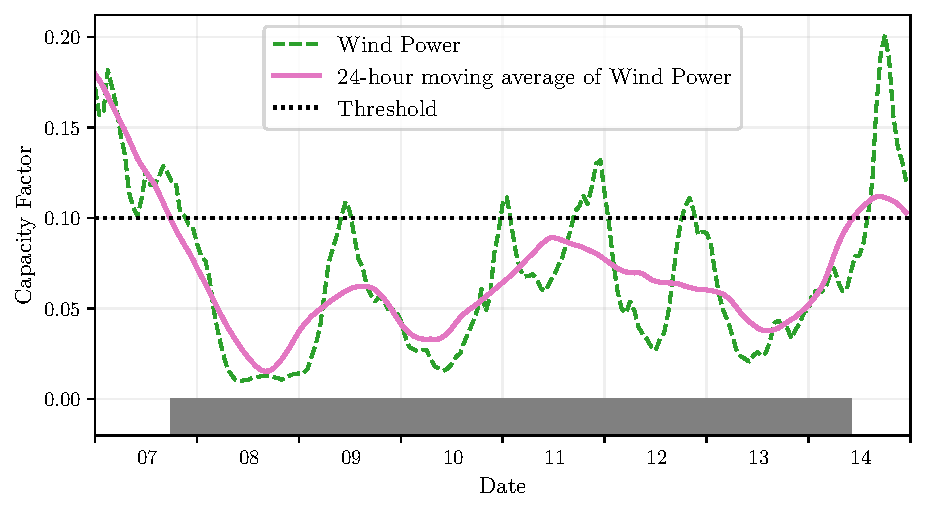
\includegraphics[width=\textwidth]{droughts_methodology.pdf}
	\caption{Wind time series of CF (green) and its 24-hour moving average (pink) from the 7th to the 15th of July 2021. The black dashed line indicates the CF threshold. The grey bar shows the period identified as a wind drought under our definition}
	\label{fig:find_res_droughts}
\end{figure}

The moving average approach smooths out short-term fluctuations, so that brief periods above the threshold do not interrupt an otherwise continuous low-CF period (Fig.~\ref{fig:find_res_droughts}). This means that a single hour above the threshold does not "break" a drought event if it is surrounded by prolonged low-generation hours. As a result, fewer but longer-lasting drought events are identified, which may better reflect real-world conditions where energy supply constraints persist over extended periods.

\section{Results}
\label{sec:Results}

\subsection{Verification}
\label{sec:verification}

The accuracy of the datasets used in this study was verified, before continuing to the analysis of RES droughts. For the verification process, time-varying values of installed capacity were used to account for changes in RES development over the verification period. This step allowed us to assess how well the datasets represent the production of renewable energy by comparing them against observed data.

\subsubsection{Wind Energy}
\label{sec:wind_verification}

The C3S-E datasets use the Vestas V136/3450 wind turbine power curve, (Fig.~\ref{fig:power_curve}a). The Atlite model allows the user to specify the power curve. We considered the 121 power curves available for download from Renewables.ninja~\citep{staffell2016wake}. For each power curve, Renewables.ninja also provides four associated smoothed power curves. The smoothing is done using a Gaussian filter with different standard deviations that depend on the wind speed. A separate wind CF time series for Ireland was generated for each of the wind turbine power curves and smoothing levels. The performance of each CF time series was then assessed based on four skill scores: correlation coefficient (CC), root mean square error (RMSE), mean bias error (MBE), and area under the curve. The area under the curve was calculated from histograms of the hourly CF values for the most recent decade, 2014-2023. Based on these metrics, the most representative power curve for Ireland was the Enercon E112.4500 power curve with the $0.3w$  smoothing filter.

\begin{figure}[!ht]
	\centering
	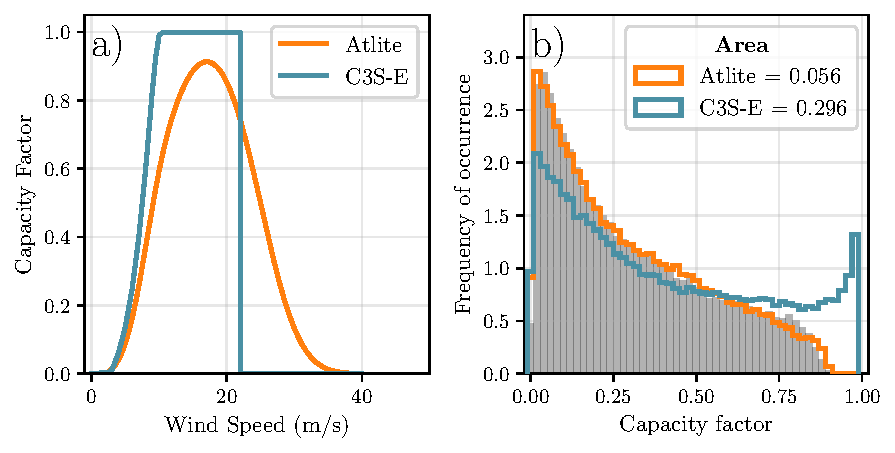
\includegraphics[width=\textwidth]{verification_power_curve.pdf}
	\caption{a) Power curves of the Enercon E112.4500 with a 0.3w smoothing filter used by Atlite (orange) and the Vestas V136/3450 used by C3S-E (blue) b) Histograms of wind CF for Ireland from Atlite (orange), C3S-E (blue) and Observed (shaded)}
	\label{fig:power_curve}
\end{figure}

The smoothing of the wind turbine power curve represents losses associated with each turbine, as well as losses such as wake effects between turbines, which are important when modelling wind energy on larger spatial scales. The histogram in Fig.~\ref{fig:power_curve}b shows that the C3S-E power curve tends to underestimate low CF values and overestimate higher ones, whereas the smoothed Atlite power curve more closely follows the recorded wind availability data from EirGrid.

\begin{figure}[!ht]
	\centering
	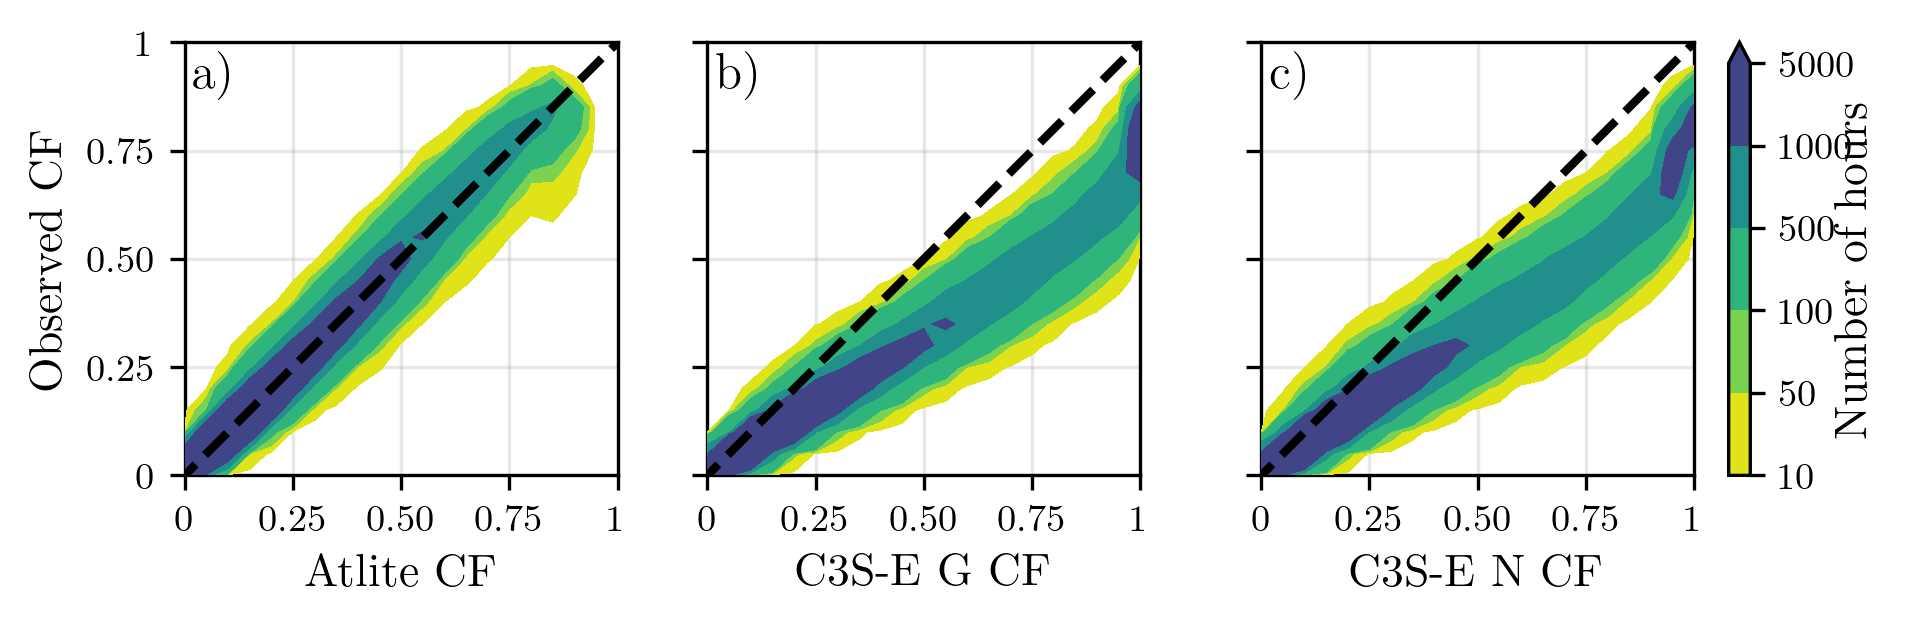
\includegraphics[width=\textwidth]{verification_wind_contour.png}
	\caption{Wind CF density plot of the observed CF (vertical axes) and modelled (horizontal axes) CF data for the a) Atlite, b) C3S-E G and c) C3S-E N models}
	\label{fig:wind_verification_contour}
\end{figure}

The effect of the difference between the power curves is also visible in Fig.~\ref{fig:wind_verification_contour}, which shows a density plot of wind CF values. The two C3S-E datasets are shown to overestimate the observed CF, whereas the Atlite model is in good agreement with the observed data. The skill scores presented in Table~\ref{tab:wind_skill_scores} show that Atlite performs better than the C3S-E datasets for all of the skill scores. 

\begin{table}[!ht]
	\centering
	\begin{tabular}{l|lll|}
		\cline{2-4}
		& \textbf{Atlite} & \textbf{C3S-E G} & \textbf{C3S-E N} \\ \hline
		\multicolumn{1}{|l|}{\textbf{CC}}   & 0.981           & 0.972            & 0.970            \\ \hline
		\multicolumn{1}{|l|}{\textbf{RMSE}} & 0.045           & 0.177            & 0.162            \\ \hline
		\multicolumn{1}{|l|}{\textbf{MBE}}   & -0.003          & 0.137            & 0.121            \\ \hline
	\end{tabular}
	\caption{Skill scores for wind power for the three datasets compared to observed data}
	\label{tab:wind_skill_scores}
\end{table}

Fig.~\ref{fig:bar_number_events_verification_wind} shows the average annual number of wind drought events during the 2014 to 2023 validation period. The figure reveals that Atlite presents the best overall agreement with the observed frequency and duration of wind drought events. This pattern is particularly evident for shorter-duration events, which are the most frequent.

\begin{figure}[!ht]
	\centering
	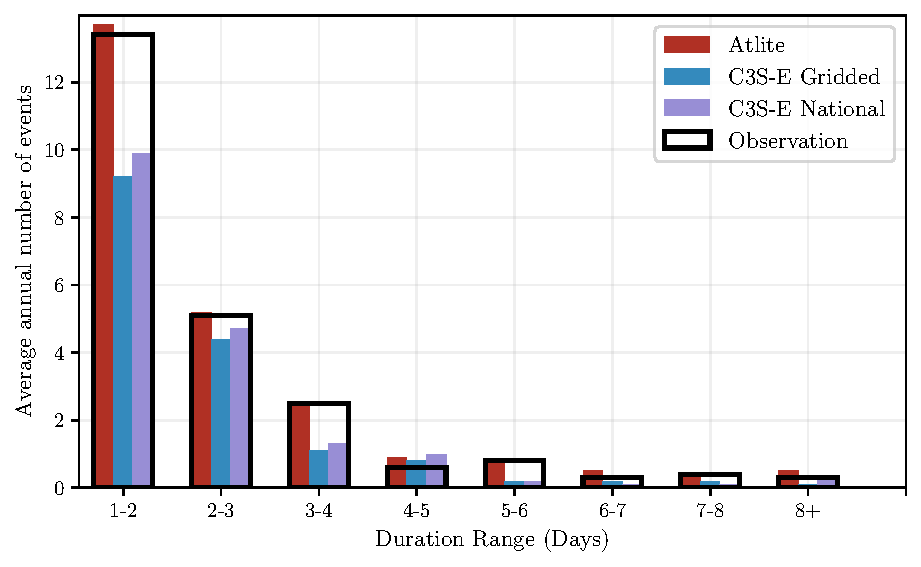
\includegraphics[width=\textwidth]{verification_wind_number_events.pdf}
	\caption{Average annual number of wind drought events for Atlite (red), C3S-E G (blue), C3S-E N (purple), and the observed data (black outline). The wind droughts are identified from 2014 to 2023, considering the actual capacity of the system at any given time}
	\label{fig:bar_number_events_verification_wind}
\end{figure}

\newpage
\subsubsection{PV Energy}
\label{sec:pv_verification}

The Atlite model allows the user to select certain PV panel characteristics. In this study, the three PV panel types available in the Atlite model were considered (CSi, CdTe, Kaneka). Following the same methodology as in the previous section, the three available models were compared using four skill scores (CC, RMSE, MB, and area under the curve). Based on the best-performing metrics, the Breyer PV panel model was selected \citep{beyer2004pv}, using the Kaneka Hybrid panel option. For all PV farm locations, the azimuth angle is fixed at 180\textdegree (due south), and the optimal tilt angle option is applied. 

The PV installed capacity available on the spreadsheets from EirGrid represents the Maximum Export Capacity (MEC) and does not accurately reflect the installed PV capacity. To enable actual PV generation potential to be modelled correctly, installed capacities were set at 1.4 times the MEC values. This scaling factor was estimated by analysing proprietary data from individual PV farms provided by EirGrid, which showed that, on average, assuming that the installed capacities of farms exceed their MEC values by 40\% yields the best agreement with the observed availability.

\begin{figure}[h!]
	\centering
	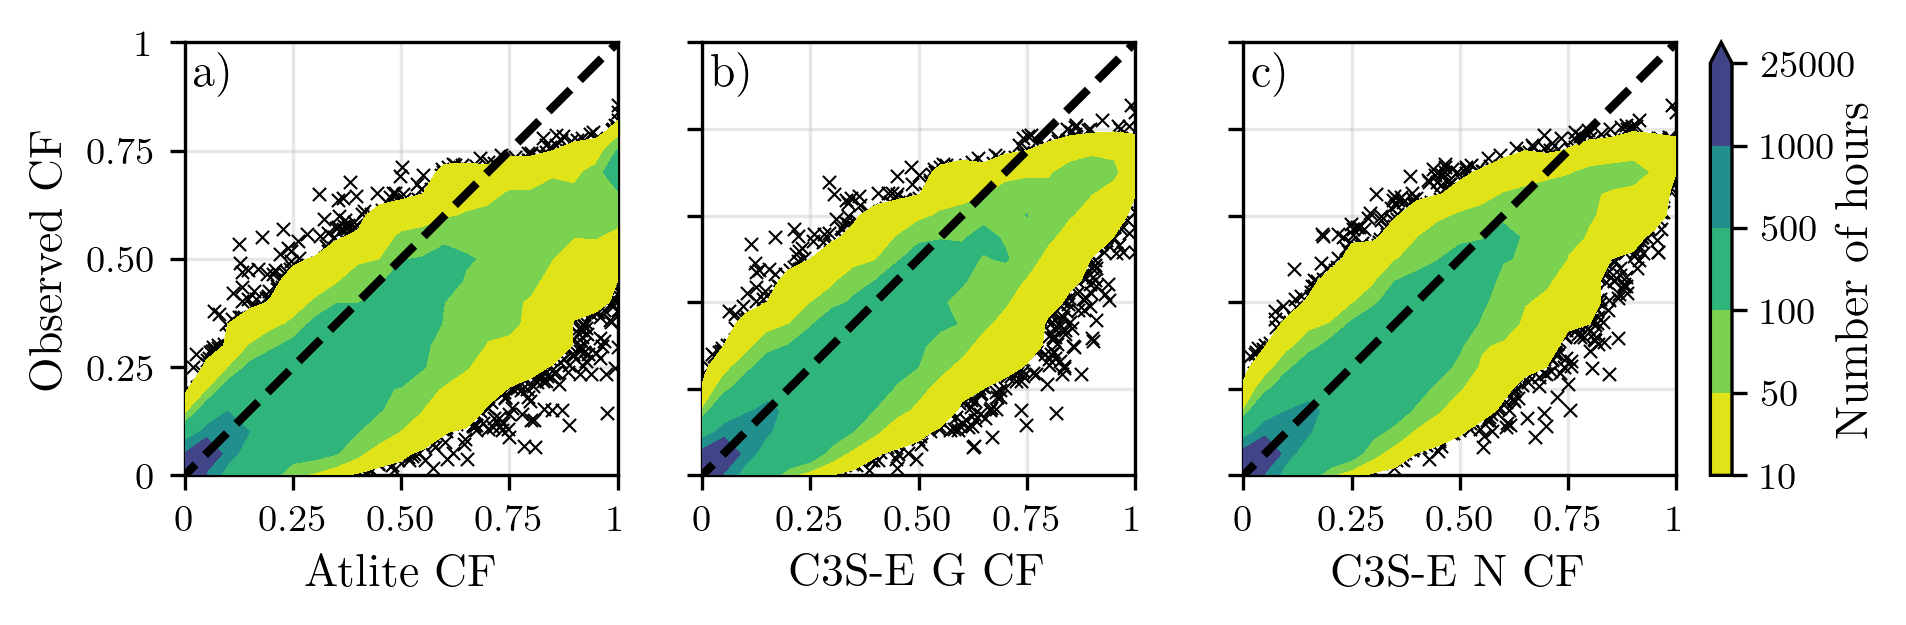
\includegraphics[width=\textwidth]{verification_pv_contour.png}
	\caption{PV CF density plot of the observed (vertical axes) and modelled (horizontal axes) CF series for the a) Atlite, b) C3S-E G and c) C3S-E N models}	
	\label{fig:solar_verification_contour}
\end{figure}

Figure \ref{fig:solar_verification_contour} shows that the three datasets have a similar tendency to overestimate the CF compared to the observed values, especially for high CF values. The skill scores presented in Table~\ref{tab:pv_skill_scores} indicate that C3S-E~G performs best overall, with the lowest RMSE and a high correlation coefficient, suggesting a closer match to observed data. All models show a slight positive bias, with Atlite exhibiting a slightly lower correlation and higher RMSE.

\begin{table}[!ht]
	\centering
	\begin{tabular}{l|lll|}
		\cline{2-4}
		& \textbf{Atlite} & \textbf{C3S-E G} & \textbf{C3S-E N} \\ \hline
		\multicolumn{1}{|l|}{\textbf{CC}}   & 0.921           & 0.931            & 0.931            \\ \hline
		\multicolumn{1}{|l|}{\textbf{RMSE}} & 0.119           & 0.090            & 0.113            \\ \hline
		\multicolumn{1}{|l|}{\textbf{MBE}}   & 0.046           & 0.027           & 0.021           \\ \hline
	\end{tabular}
	\caption{Skill scores for PV CF for the three datasets compared to observed data}
	\label{tab:pv_skill_scores}
\end{table}

Fig.~\ref{fig:bar_number_events_verification_pv} shows the number of PV drought events during the 2023 validation period across different duration ranges. The figure reveals partial agreement between the three datasets and the observed data, with consistent results noticed for duration ranges of 1-2, 3-4, 7-8, and 8+ days. However, discrepancies appear in the other ranges, where the models diverge from the observed data. The main challenge in validating PV data stems from the recent installation of a large share of Ireland’s PV capacity, leading to uncertainties in PV generation data and the actual generating capacity in the first few months after each farm is connected. With over 65\% of the total PV capacity installed in 2023, these data uncertainties significantly impact the ability to perform rigorous validation for PV drought events. 

Nevertheless, the goal of this analysis is to assess the combination of wind and PV generation, where the complementary nature of these energy sources mitigates the limitations seen in PV-only results.

\begin{figure}[!ht]
	\centering
	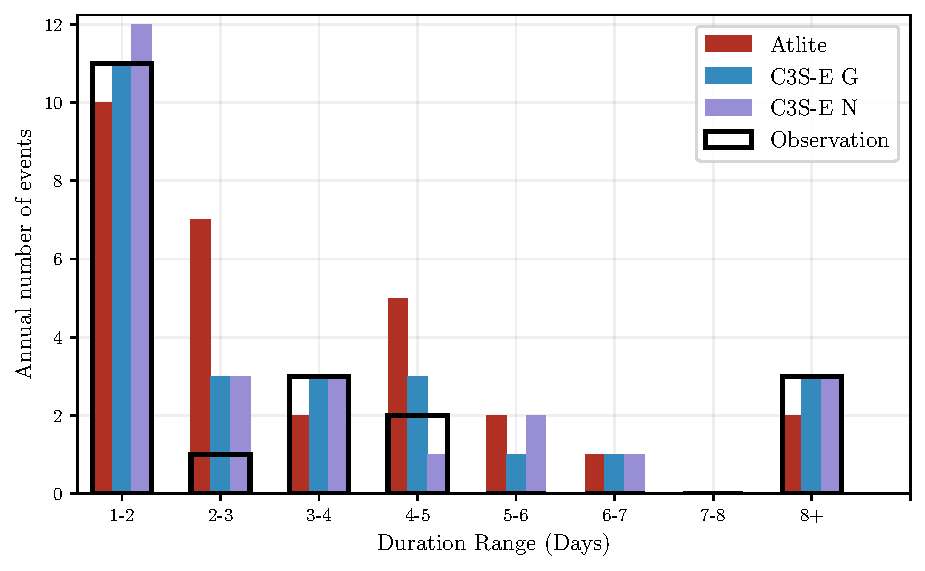
\includegraphics[width=\textwidth]{verification_pv_number_events.pdf}
	\caption{Number of PV drought events for Atlite (red), C3S-E G (blue), and C3S-E N (purple) and the observed data (black outline). The PV droughts are identified for 2023, considering the actual capacity of the system at any given time}
	\label{fig:bar_number_events_verification_pv}
\end{figure}

\newpage
\subsection{Analysis}
\label{sec:Analysis}

In this section, RES drought events are evaluated under two different scenarios with fixed installed capacities: the 91W-9PV scenario, with 5.9 GW of wind capacity and 0.6 GW of PV capacity; and the 57W-43PV scenario, where wind capacity comprises 11.45 GW and PV capacity increases to 8.6 GW. Both scenarios were driven by 45 years of ERA5 data. Using the RES drought identification process described in Section~\ref{sec:res_drought}, wind and PV droughts are first analysed separately before presenting the results for combined (wind + PV) RES droughts under both scenarios.

\subsubsection{Annual Number of RES Droughts}

The first part of the analysis examines the annual number of RES drought events across the three datasets. When only wind energy is considered (Fig.~\ref{fig:boxplot_number_events}a), the number of events decreases as the duration range increases, with very few events lasting more than seven days. In the case of only PV energy (Fig.~\ref{fig:boxplot_number_events}b), the number of events also declines as the duration range extends from one to eight days, followed by a slight increase for longer durations. This increase is due to extended low-generation periods occurring from November to March, depending on the dataset. When comparing wind and PV results (Fig.~\ref{fig:boxplot_number_events}a~\&~b), the median, first, and third quartiles for PV are consistently higher than or equal to those for wind, across all duration ranges and datasets. This is due to the typically lower CF of PV power compared to wind power, especially in a region such as Ireland where solar potential is limited. PV generation is also zero at night and constrained by the daily solar cycle, leading to a naturally higher frequency of drought events in PV compared to wind.

Fig.~\ref{fig:boxplot_number_events}c~\&~d show the combination of wind and PV under the two capacity scenarios. In the 91W-9PV scenario (Fig.~\ref{fig:boxplot_number_events}c), the identified RES droughts closely match those for wind alone, which is expected due to the dominance of installed wind capacity. In contrast, the 57W-43PV scenario (Fig.~\ref{fig:boxplot_number_events}d) shows a clear reduction in the number of drought events across all datasets and durations, with a decrease of the total number of events of 56\% for Atlite, 52\% for C3S-E G, and 50\% for C3S-E N. This reduction is attributed to the anti-correlation between wind and PV generation.

The median, first, and third quartiles for the Atlite dataset are consistently greater than or equal to those of the other two datasets, regardless of the duration range or type of renewable energy considered. This difference arises from the wind turbine power curve model used in the C3S-E datasets, which tends to overestimate the wind CF (Fig.~\ref{fig:wind_verification_contour}). As a result, the overall number of RES droughts is underestimated in the C3S-E datasets compared to Atlite. 

\begin{figure}[!ht]
	\centering
	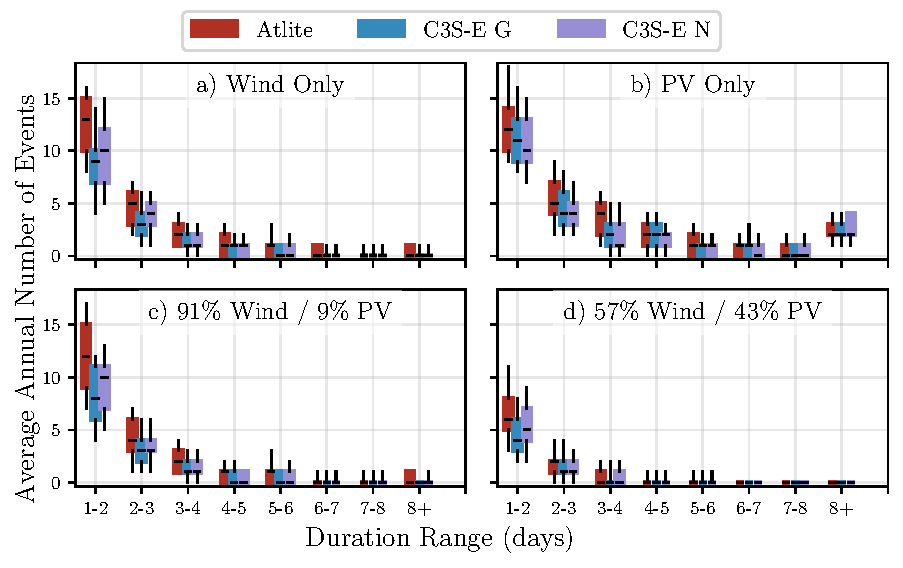
\includegraphics[width=\textwidth]{droughts_number_events.pdf}
	\caption{Annual number of RES droughts (from 1979 to 2023) for a)~Wind, b)~PV, and the combination for the c)~91W-9PV and d)~57W-43PV scenarios for Atlite (red), C3S-E G (blue), and C3S-E N (purple). The x-axis represents duration ranges in days (lower bound included), while the y-axis indicates the annual number of events. The boxes display the first and third quartiles and the median is marked by a black line. The whiskers indicate the 5th and 95th percentiles}
	\label{fig:boxplot_number_events}	
\end{figure}

\newpage
\subsubsection{Return Periods of RES Drought Duration}

The RES drought events identified over the 45-year period were used to calculate the return periods for different RES drought durations. A return period is the estimated average time interval between events of a specified duration or intensity (not to be confused with the frequency of their occurrence within a fixed time frame). Fig.~\ref{fig:return_periods} illustrates the return periods for varying RES drought durations, highlighting how often different drought lengths are likely to occur across the datasets. This analysis provides insight into the frequency and likelihood of prolonged low-generation periods, which is crucial for evaluating the potential impact of RES droughts on energy reliability and security of supply.

The duration of wind droughts (Fig.~\ref{fig:return_periods}a) increases in a log-linear fashion across the three datasets. The log-linear trend indicates a predictable relationship between drought duration and occurrence, with longer wind droughts becoming exponentially less likely as duration increases. 

In the case of PV droughts (Fig.~\ref{fig:return_periods}b), Atlite behaves differently than the two C3S-E datasets. The Atlite results show a log-linear increase but reach higher values in general with the longest event lasting forty days. For C3S-E G and C3S-E N, the duration of PV droughts increases in a log-linear pattern for events lasting less than 16 days. Beyond this duration, there is a sharp rise in drought duration for events up to a one-year return period. This sudden increase reflects the impact of winter on PV generation in Ireland, as PV output often remains below the CF threshold for extended periods during winter months. The difference between Atlite and the C3S-E results arises from differences in the datasets near the threshold of 0.1 CF. Atlite remains slightly above the threshold more frequently during these conditions, leading to shorter, more fragmented drought events. In contrast, C3S-E G and C3S-E N tend to fall below the threshold in similar conditions, resulting in longer continuous drought periods, especially during winter. This sensitivity to the threshold highlights how slight model differences can have substantial effects on drought duration estimates, particularly for PV in low-generation conditions.

For the 91W-9PV scenario (Fig.~\ref{fig:return_periods}c), the return periods mirror those of Fig.~\ref{fig:return_periods}a, due to the low levels of installed PV capacity. In the 57W-43PV scenario (Fig.~\ref{fig:return_periods}d), the return periods for RES droughts increase across all durations. For example, the return period for a five-day drought event (shown by the vertical dashed lines in Fig.~\ref{fig:return_periods}) extends from roughly six months for the 91W-9PV scenario, to four years for the 57W-43PV scenario in the Atlite dataset, and from about fifteen months to around five years in the two C3S-E datasets.

\begin{figure}[!ht]
	\centering
	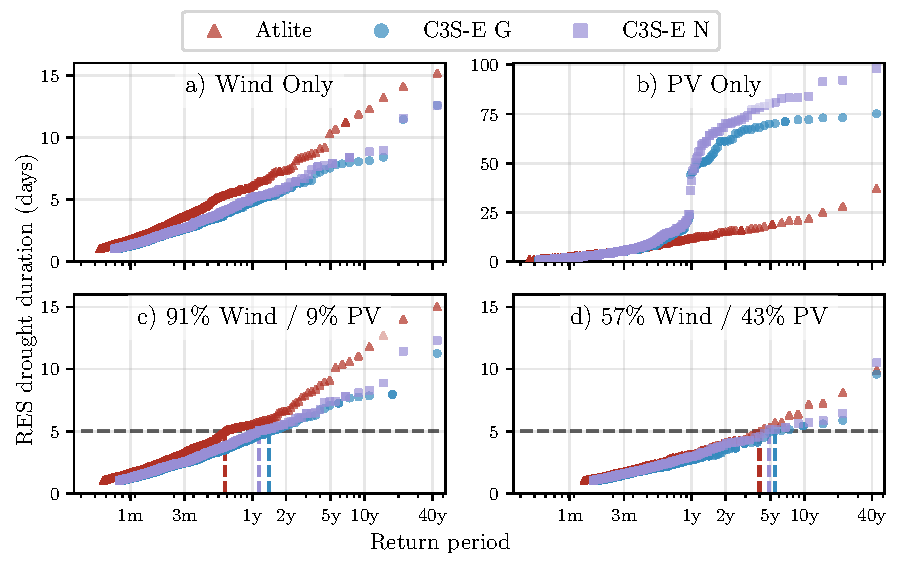
\includegraphics[width=\textwidth]{droughts_return_periods.pdf}
	\caption{Return periods of the duration of RES droughts  (from 1979 to 2023) for a)~Wind, b)~PV, and the combination for the c)~91W-9PV and d)~57W-43PV scenario, for Atlite (red triangle), C3S-E G (blue circle), and C3S-E N (purple square). The x-axis represents the return period time in a log-scale and the y-axis indicates the duration of RES drought associated with it. The horizontal dashed line marks the 5-day return period, with coloured vertical dashed marking its return period for each dataset}
	\label{fig:return_periods}
\end{figure}

Across Fig.~\ref{fig:return_periods}a, c, and, d, the return periods in the Atlite dataset are consistently higher than those in the two C3S-E datasets. For instance, in the 91W-9PV scenario (Fig.~\ref{fig:return_periods}c), an event with a one-year return period lasts six days in the Atlite dataset, compared to only five days in the C3S-E datasets. This difference underscores the importance of model selection when quantifying RES droughts, as each model’s assumptions and parametrisations significantly influence drought duration estimates. Additionally, in all four graphs, the similarity between results from the two C3S-E datasets suggests that assumptions in the Atlite model—such as wind turbine power curve selection and PV panel specifications—have a greater impact on RES drought duration estimates than the precise geographic distribution of RES farms when studying the return periods of RES droughts.

\newpage
\subsubsection{Seasonal Distribution of RES Droughts}

The seasonality of RES droughts was analysed by comparing the percentage of hours in each month classified as part of a RES drought. 

The percentage of hours that are part of a wind drought (Fig.~\ref{fig:res_droughts_seasonality}a) are higher in summer than in winter. In the Atlite dataset, for instance, an average of 24\% of hours in summer (June-July-August) are identified as wind droughts, compared to only 4\% in winter (December-January-February). This seasonal variation is less prominent for the two C3S-E datasets compared to the Atlite one. This difference can be linked to the shape of the two power curves (Fig.~\ref{fig:power_curve}). CFs near or under the 0.1 threshold are produced by higher wind speeds for the Atlite power curve than for the C3S-E one. In contrast, the results for PV droughts (Fig.~\ref{fig:res_droughts_seasonality}b) show a higher percentage in winter, with PV droughts occurring over 60\% of the time regardless of the dataset. The Atlite results show a higher percentage of PV drought hours for wind, and a slightly lower percentage for PV, compared to the two C3S-E datasets. 

\begin{figure}[!ht]
	\centering
	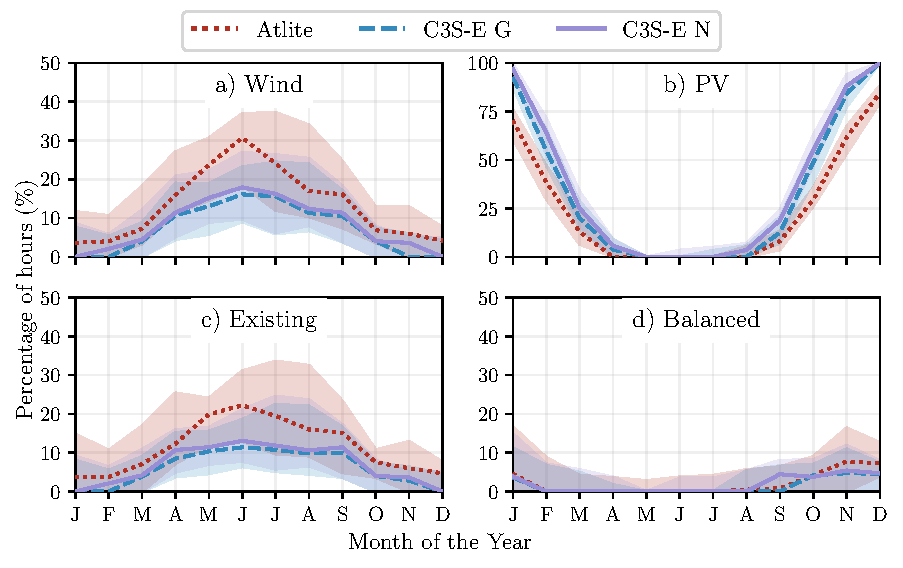
\includegraphics[width=\textwidth]{droughts_seasonality.pdf}
	\caption{Percentage of hours in a month which are part of a RES drought (from 1979 to 2023) for a)~Wind, b)~PV, and the combination for the c)~91W-9PV and d)~57W-43PV scenario, for Atlite (red dotted), C3S-E G (blue dashed), and C3S-E N (purple solid). The x-axis represents the month of the year, and the y-axis indicates the percentage of hours. Lines correspond to the median values and the area between the first and third quartiles is shaded.}
	\label{fig:res_droughts_seasonality}
\end{figure}

Similar to previous results, the 91W-9PV scenario (Fig.~\ref{fig:res_droughts_seasonality}c) shows patterns comparable to the ones for wind droughts (Fig.~\ref{fig:res_droughts_seasonality}a). However, in the 91W/9PV scenario, the number of hours classified as RES droughts in summer decreases slightly compared to the wind-only scenario. This reduction can be explained by the contribution of PV generation during the summer months in the 91W-9PV scenario, even though it constitutes only 11\% of total capacity. Since the number of RES drought hours for PV in summer is near zero, this small contribution has a noticeable impact on reducing overall drought hours. In the 57W-43PV scenario (Fig.~\ref{fig:res_droughts_seasonality}d), all three datasets show a reduction in monthly RES drought frequency. Annual reductions in median RES drought frequency are observed across the datasets, dropping from 14\% to 5\% for Atlite, from 8\% to 3\% for C3S-E G, and from 9\% to 4\% for C3S-E N. The balanced mix of wind and PV power in this scenario reduces the seasonal signal overall and significantly decreases the percentage of RES drought hours in the summer.

\newpage
\section{Discussion and Conclusions}
\label{sec:Conclusion}

This study has investigated the ability of three RES models to represent RES droughts: Atlite, C3S-E G, and C3S-E N. One of the most evident differences is how each dataset incorporates the specific locations of RES farms. Both Atlite and C3S-E G consider the locations of wind and PV farms, which should, in theory, provide a more accurate representation of RES generation. While this approach slightly improves PV models, our analysis indicates that for wind energy, the Atlite dataset performs better overall, especially in its close alignment with observed data for wind generation estimates. This finding suggests that, although the inclusion of RES farm locations is beneficial, the accuracy of the RES model is more strongly influenced by underlying model assumptions, such as selecting an appropriate wind power curve.

Atlite shows the best alignment with observed data for wind generation. Differences between the models are smaller for PV, with C3S-G performing marginally better than the other two. The results show that the two C3S-E datasets (C3S-E G and C3S-E N) consistently yield similar outcomes, indicating that their methodological differences have minimal impact. This distinction was also evident in the analysis, where Atlite reported higher return periods and a greater number of RES droughts, especially in scenarios with a balanced share of RES. Again, the results from RES drought modelling rely more on the precision of the wind power curve and PV panel models than on the specific locations of RES farms. Atlite’s superior performance highlights the importance of selecting validated models for assessing RES drought risks. This careful model selection can better quantify risks, support effective planning, and avoid the potential underestimation of capacity needs, which is essential for ensuring energy security.

Looking at the 57W-43PV scenario, the analysis showed a significant improvement in the management of RES droughts due to the complementary nature of wind and PV generation. Wind and PV together perform better in terms of reducing drought frequency and duration than either would individually, largely because of the seasonal anti-correlation between the two energy sources. This diversification reduces the seasonal impact on RES droughts, as PV generation peaks in the summer and wind generation is more consistent in winter. Ireland currently has a highly wind-dependent energy system, but with ambitious targets for PV installations in the coming years, the energy mix is expected to approach a balance between wind and PV capacity. While this balanced approach offers a more stable and secure energy supply by mitigating RES drought risks, it is important to note that having similar wind and PV capacities may not optimise other aspects, such as annual energy production or meeting nighttime loads. For policymakers, these findings underscore the importance of meeting these capacity targets to enhance energy security through diversification. Additionally, the choice of model for RES drought assessment becomes increasingly critical as more renewable capacity is integrated into the system.

Future work is planned to extend the current analysis. First, climate projection data will be integrated with different energy scenarios, incorporating the addition of offshore wind, to better understand how climate change might affect RES droughts. Second, expanding the geographic domain of the study to include the rest of Europe would provide a more comprehensive understanding of RES droughts in an interconnected energy grid. This would require extensive verification across other European countries, making it a more complex but highly relevant challenge.

\section*{Data Availability}

The ERA5 data can be obtained from the Climate Data Store (\url{https://doi.org/10.24381/cds.adbb2d47}). The C3S-E dataset is also available from the Climate Data Store (\url{https://doi.org/10.24381/cds.4bd77450}). Information on wind and PV farms in Ireland can be obtained from the EirGrid website (\url{https://www.eirgrid.ie/grid/system-and-renewable-data-reports}). The Atlite model used in this study is open-source and can be found on GitHub (\url{https://github.com/pypsa/atlite}). The data and code required to reproduce the analysis in this article will be made available upon acceptance of the manuscript in a public GitHub repository.

\section*{Acknowledgments}

The research conducted in this publication was funded by Science Foundation Ireland and co-funding partners under grant number 21/SPP/3756 through the NexSys Strategic Partnership Programme.

\bibliographystyle{elsarticle-num-names}
\bibliography{RES_droughts_Morin_ref}

\end{document}

\endinput



